\section{}
The metronome shown is used as a timing device for musicians. The essence of the device is an
inverted 'T' mounted on springs. The natural frequency of the device is varied by moving the mass
$m$ to different heights $L$.

Assuming that the system undergoes only small oscillations about the axis through point $O$ (the
static equilibrium configuration is at $\theta = 0$):
\begin{enumerate}[label=(\alph*)]
    \item (5 pts) Determine the equation of motion of the system using $\theta$ as your coordinate.
        Neglect the mass of the 'T' bar. Be sure to include the force of gravity as there is no
        static deflection of the springs in the static equilibrium configuration.
    \item (5 pts) What is the limiting value of $L$ so that the system is stable?
\end{enumerate}

\subsection*{Solution}  
\subsection{}
\begin{figure}[h]
    \centering
    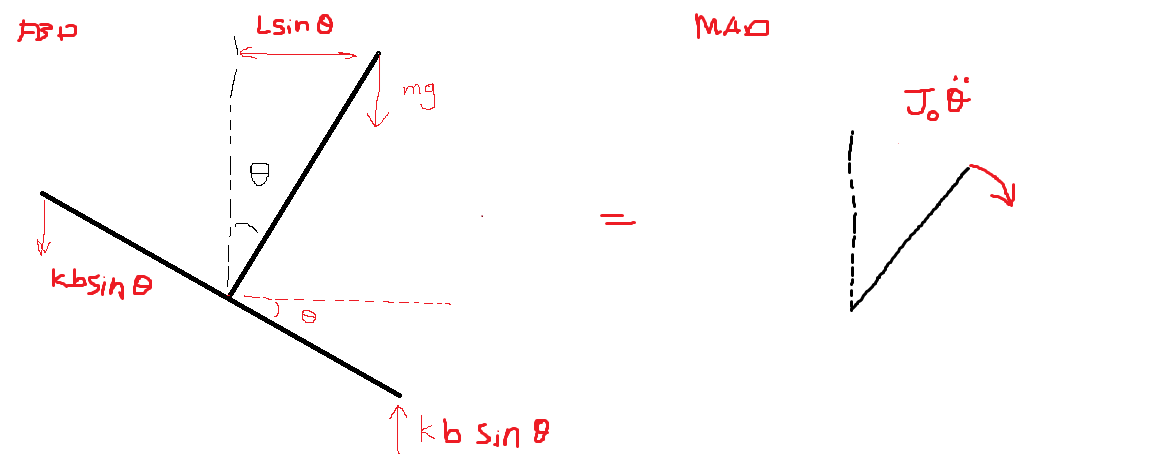
\includegraphics[width=0.7\linewidth]{Questions/Figures/q1 fbd.png}
    \caption{The metronome system}
    \label{fig:q1_fbd-png}
\end{figure}
From the free body diagram and mass acceleration diagram, we can take the moment about the 
pivot point $O$ to get the equation of motion:
\begin{gather*}
    \circlearrowright \sum M_O = J_O \ddot{\theta} \\
    \implies -k (b\sin\theta) (b \cos \theta) - k (b\sin\theta)(b \cos \theta) + mg L \sin \theta = J_O \ddot{\theta} \\
    \implies -2kb^2 \sin\theta \cos\theta + mgL \sin\theta = mL^2 \ddot{\theta} \\
    \implies -\frac{2kb^2}{mL^2}\cos\theta \sin\theta + \frac{g}{L} \sin\theta = \ddot{\theta}
\end{gather*}
So the equation of motion is:
\begin{align*}
    \Aboxed{\ddot{\theta} + \left(\frac{2kb^2}{mL^2}\cos\theta - \frac{g}{L}\right) \sin\theta &= 0}
\end{align*}
\subsection{}
Applying linearization, we get:
\begin{align*}
    \ddot{\theta} + \left(\frac{2kb^2}{mL^2} - \frac{g}{L}\right) \theta &= 0
\end{align*}
From differential equations, the solution is bounded if the roots of the characteristic equation have negative real parts. Therefore,
\begin{align*}
    \frac{2kb^2}{mL^2} - \frac{g}{L} &\geq 0 \\
    \Aboxed{L &\leq \frac{2kb^2}{mg}}
\end{align*}